
\documentclass[english]{article}

\usepackage{graphicx}
\usepackage{grffile}
\usepackage{babel}
\usepackage{parskip}
\textwidth = 426pt
\oddsidemargin = 17pt


\title{Coding standards document\\}
\date{\today}


\begin{document}
	\maketitle
	


	\section{Style,Structure and layout}
			

		\subsection{Variables, Methods and attributes:}
			$\bullet$\ Should be short and descriptive.\par
			$\bullet$\ Should begin with lower-case letter.\par
$\bullet$\ Upper-case letter should be used immediately after the first name description of the variable.\par
$\bullet$\ Should use a single upper-case letter at the start of each new word within the name.\par
$\bullet$\ Should not be a single character e.g. string x  \par


                                	

		\subsection{Accessor and Mutators}
$\bullet$\  Should have names based on the attribute to which they provide access.\par
$\bullet$\ Should begin with the prefix “get” or “set” followed by the name of the attribute beginning with a capital letter e.g. getItem \par

		\subsection{Final variables}
		$\bullet$\ Should make use of final variables instead of magic numbers to avoid making it hard to identify which numbers should be changed if the use of the program needs to be altered.\par
			$\bullet$\ Should have all upper-case names to make them clearly identifiable.\par		
				
				
		\subsection{Indentation and Layout}
		$\bullet$\ Blocks that are nested more should be indented more. \par
		
$\bullet$\ Lines should be kept to a sensible length to make the code easier to read and print.\par	
	$\bullet$\ Single blank lines should be used to separate methods and to emphasise blocks of code.\par	
		
				\subsection{Bracketing}
$\bullet$\ Brackets will be used to clearly show the blocks of code they encapsulate.\par
$\bullet$\ Closing curly brackets should be placed on the line after the last line of the code they enclose, at the same level of indentation as the start of the header on which the block begins. \par
$\bullet$\ Curly brackets should always be used for if-, while- and for-, even when not strictly needed – such as when the body only contains a single statement.\par
\subsection{Exceptions}
$\bullet$\ Exceptions should be used where necessary.\par
$\bullet$\ Instead of throwing basic Exception classes, sub-classes should be made with more meaningful names.\par
$\bullet$\ Appropriate “catch” statements should be put in place to allow the program to recover if need be.\par




\subsection{Imports}
$\bullet$\ Should avoid using import *(importing every package), rather each class should be specifically imported as required.\par

$\bullet$\ Any unused imports should be removed if they are no longer needed to make it clear which classes will be used.\par


				
			\section{Naming Conventions	}
			This section will cover examples referring to some of the conventional rules mentioned above.
				
					\subsection{ Classes }
$\bullet$\ Class names should begin with a capital letter and each new word within the name should begin with a capital letter e.g "ClassName".\par

				\subsection{Exception Classes}
$\bullet$\ Exception classes should follow the same rule as normal classes, but should end with the word Exception e.g "ClassNameException ".\par
\subsection{Methods}
$\bullet$\ Methods should begin with a lower case letter and each new word within the name should begin with a capital letter e.g "methodName()".\par
\subsection{Variables and Attributes }
$\bullet$\ Both variables and attributes should being with a lower case letter and each new word within the name should begin with a capital letter – exactly the same as methods e.g "variableName".\par
\subsection{Packages}
$\bullet$\ Package names should all be in lower case e.g "demo.package".\par

	\section{XML	}
	
	\subsection{Tags}
$\bullet$\ XML tags should be ordered as follows: "xmlns" first, then id,then  \texttt{layout\_width} and  \texttt{layout\_height} alphabetically. \par
$\bullet$\ Add a space between the closing slash and the final attribute.\par E.g.  \texttt{android:textSize="10dp" /> }\par
$\bullet$\ Self closing tags should be used when an XML element doesn't have any contents, you should use self closing tags. \par

\subsection{Layout XML ID Naming / Java Class Widget Declaration Variable}
				
This section provides a guide on how to use elements and prefixes.
				\\
				\begin{tabular}{ |p{3cm}|p{9cm}|  }
				\hline
				\textbf{Element} & \textbf{Prefix And Example}  \\
				\hline
				
				TextView &	tv	e.g tvText\\
				\hline
				ImageView &	iv	e.g ivImage\\
				\hline
				Button &	btn	e.g btnSubmit\\
				\hline
				EditText &	et	e.g etWords \\
				\hline
				\end{tabular}

\section{Documentation}

\subsection{Comments}
$\bullet$\ Use in-line commenting to help the next developer who might be editing your code.\par
$\bullet$\ Inline comments should appear on the line above the code you are commenting.\par
$\bullet$\ Comment XML View elements using  \texttt{<! -- Comment -->}.\par
$\bullet$\ Comments should be added within the body of a method if they are used within that method.\par



\subsection{Resource Files}
$\bullet$\ Resources file names should be written in  \texttt{lowercase\_underscore}  e.g  \texttt{ic\_star.png} \par


\subsection{Layout Files}

$\bullet$\ Layout files should match the name of the Android components that they are intended for but moving the top level component name to the beginning. \par
$\bullet$\ Example, if you are creating a layout for the SignInActivity, the name of the layout file should be \texttt{activity\_sign\_in.xml} \par


\subsection{Version control}
$\bullet$\ No commented out code must be committed unless you have a very good reason that is clearly described in a comment by the code you are committing. \par


\section{Repository}


\begin{figure}[ht!]
\centering
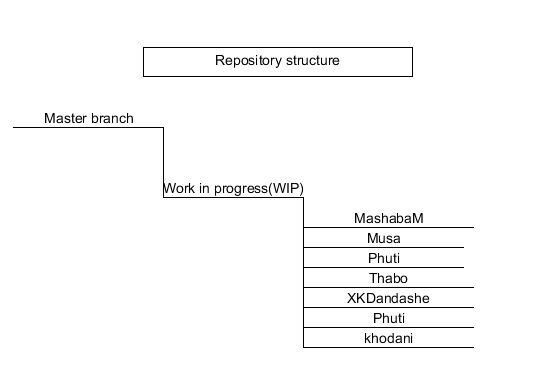
\includegraphics[width=90mm]{repo.png}
\caption{Repository structure }
\end{figure}				

\subsection{Repository definitions}
$\bullet$\ All the pictures should be in a folder called Pictures. \par
$\bullet$\ All the files should belong to a specific folder. \par
$\bullet$\ Folder names should be descriptive enough to show what they contain. \par
$\bullet$\ The diagram below shows the structure of the repository. \par





















		\subsection{References}
\begin{itemize}
			\item https://source.android.com/setup/contribute/code-style\\
			\item https://github.com/ekimual/android-coding-standards
		\end{itemize}
		


\end{document}
